\documentclass[12pt,a4paper]{report}
\usepackage[utf8]{inputenc}
\usepackage{amsmath}
\usepackage{amsfonts}
\usepackage{amssymb}
\usepackage{graphicx}
\usepackage{chemstyle}
\usepackage{mdframed}
\usepackage{tikz}
\usetikzlibrary{matrix}
\addtolength{\topmargin}{-1in}
\setlength{\textwidth}{6.3in}
\setlength{\textheight}{9.5in}
\newcommand*\diff{\mathop{}\!\mathrm{d}}
\newcommand{\overbar}[1]{\mkern 1.5mu\overline{\mkern-1.5mu#1\mkern-1.5mu}\mkern 1.5mu}

% code to hide part of the text leaving the blank space in its place
\ExplSyntaxOn
\box_new:N \l_mypkg_box
\int_new:N \l_mypkg_cleanup_int
\DeclareDocumentCommand{\hideit}{O{1}+m}
  {
    \tex_setbox:D \l_mypkg_box \tex_vbox:D
      {
        #2\par
        \dim_zero:N \tex_baselineskip:D
        \dim_zero:N \tex_lineskip:D
        \dim_zero:N \tex_lineskiplimit:D
        \int_set:Nn \l_mypkg_cleanup_int {#1}
        \mypkg_dismantle_loop:
      }
    \tex_unvbox:D \l_mypkg_box
  }
\cs_new_protected:Npn \mypkg_dismantle_loop:
  {
    \prg_replicate:nn { \l_mypkg_cleanup_int }
      {
        \skip_if_eq:nnT { \tex_lastskip:D } { \c_zero_skip } { \tex_unskip:D }
        \dim_compare:nT { \tex_lastkern:D = \c_zero_dim } { \tex_unkern:D }
        \int_compare:nT { \tex_lastpenalty:D = \c_zero } { \tex_unpenalty:D }
      }
    \skip_if_eq:nnTF { \tex_lastskip:D } { \c_zero_skip }
      {
        \dim_compare:nTF { \tex_lastkern:D = \c_zero_dim }
          {
            \int_compare:nTF { \tex_lastpenalty:D = \c_zero }
              {
                \box_set_to_last:N \l_mypkg_box
                \box_if_empty:NF \l_mypkg_box
                  { \mypkg_dismantle_box: }
              }
              { \mypkg_dismantle_penalty: }
          }
          { \mypkg_dismantle_kern: }
      }
      { \mypkg_dismantle_skip: }
  }
\cs_new_protected:Npn \mypkg_dismantle_skip:
  { \mypkg_dismantle_aux:nN { \tex_vskip:D \skip_use:N \tex_lastskip:D } \tex_unskip:D }
\cs_new_protected:Npn \mypkg_dismantle_kern:
  { \mypkg_dismantle_aux:nN { \tex_kern:D \dim_use:N \tex_lastkern:D } \tex_unkern:D }
\cs_new_protected:Npn \mypkg_dismantle_penalty:
  { \mypkg_dismantle_aux:nN { \tex_penalty:D \int_use:N \tex_lastpenalty:D } \tex_unpenalty:D }
\cs_new_protected:Npn \mypkg_dismantle_box:
  { \mypkg_dismantle_aux:nN { \tex_vbox:D to \dim_eval:n { \box_ht:N \l_mypkg_box + \box_dp:N \l_mypkg_box } { } } \scan_stop: }
\cs_new_protected:Npn \mypkg_dismantle_aux:nN #1#2
  {
    \use:x
      {
        #2
        \mypkg_dismantle_loop:
        #1 \scan_stop:
      }
  }
\ExplSyntaxOff

%conditional compilation for students version of document
\newif\ifstudents
%\studentstrue % comment out to hide text and equations

\begin{document}
   \pagestyle{headings}
   \thispagestyle{plain}
   \newpage
   \noindent
   \begin{center}
   \framebox{
       \vbox{
           \hbox to 6in { {\bf CHM2003 Physical Chemistry 2 \hfill October 2013} }
           \vspace{4mm}
           \hbox to 6in { {\Large \hfill Thermodynamics   \hfill} }
           \vspace{2mm}
           \hbox to 6in { {\it Giuliano Maurizio Laudone \hfill Lecture 2} }
      }
   }
   \end{center}
   \section*{Liquid solutions}
   \subsection*{Ideal and real solutions}
   So far we focused only on systems containing a single component. Now we'll begin the study of multi-component systems and we'll discuss and quantify the effects of their chemical composition. 
   The first such system that we'll study is a binary liquid solution in equilibrium with its vapour. 
   \begin{figure}[H]
   \begin{center}
   \includegraphics[scale=0.3]{Images/Lect2_binary_solution.pdf} 
   \end{center}
   \end{figure}
   When working with gases, we initially defined a limiting case, an ideal gas, with a behaviour that could be easily described mathematically and to which real gases could be approximated under certain conditions. Similarly we'll now define an \textit{ideal solution}.
   It was found experimentally by Raoult that in certain binary solutions (usually those made of relatively similar molecules) the partial vapour pressure of each component is proportional to the molar fraction of each species in the liquid phase:
   \ifstudents \hideit[2]{ \fi
   \begin{equation*}
   p_{i}=x_{i}p^{*}_{i}
   \end{equation*}
   \ifstudents } \fi
   where $p^{*}_{i}$ is the vapour pressure of pure component $i$ of the solution. A solution in which all components follow Raoult's law at any value of molar fraction is called an ideal solution.
   \begin{center}
   \begin{tikzpicture}[scale=2]
	\draw (-2.5,2) -- (-2.5,-3) node (v1) [below]{$0$} -- (1.5,-3) node (v2) [below]{$1$} -- 		(1.5,2);
	\draw[dashed](-2.5,-3) -- node[midway,below] {$p_{\mathrm{A}}$}(1.5,-1) node [right]			{$p^{*}_{\mathrm{A}}$};
	\draw[dashed](1.5,-3) to node[midway,below] {$p_{\mathrm{B}}$}(-2.5,1) node [left]				{$p^{*}_{\mathrm{B}}$};
	\draw[-] (-2.5,1)to node[midway,above] {$p$} (1.5,-1);
	\node at (-0.5,-3) [below]{$x_{\mathrm{A}}$};

	\node at (1.5,-2) {};
	\end{tikzpicture}
   \end{center}
   Few solutions, such as, for example, benzene-toluene solutions, are found to be fairly close to an ideal solution, while other solutions show large deviations from the ideal behaviour. However, even for such solutions one of the components, the solvent, as its molar fractions tends to 1 (pure solvent) its experimental behaviour approximates Raoult's law.
   
   Henry's law was derived experimentally for very dilute solution is and it can be expressed as:
   \ifstudents \hideit[2]{ \fi
   \begin{equation*}
   p_{i}=x_{i}K_{i}
   \end{equation*}
   \ifstudents } \fi
   The vapour pressure of component $i$ is proportional to its molar fraction in the liquid phase, but the proportionality constant is not the vapour pressure of the pure substance, but a different proportionality constant $K_{i}$, which is called Henry's constant. 
   \begin{center}
   \begin{tikzpicture}[scale=1.5]
	\draw (-2.5,2) -- (-2.5,-3) node (v1) [below]{$0$} -- (1.5,-3) node (v2) [below]{$1$} -- (1.5,2);
	\draw[dashed](-2.5,-3) -- node[sloped,midway,below] {Raoult's law}(1.5,-1) node [right] (v3) {$p^{*}_{\mathrm{A}}$};
	\draw[dashed](-2.5,-3) -- node[sloped,midway,above] {Henry's law}(1.5,1.5) node [right]{$K_{\mathrm{A}}$};
	\node at (-0.5,-3) [below]{$x_{\mathrm{A}}$};
	\node at (1.5,-2) {};
	\draw (-2.5,-3);
	\draw (-2.5,-3) .. controls (0,-0.1) and (0.5,-1.5) .. (1.5,-1);
   \end{tikzpicture}
   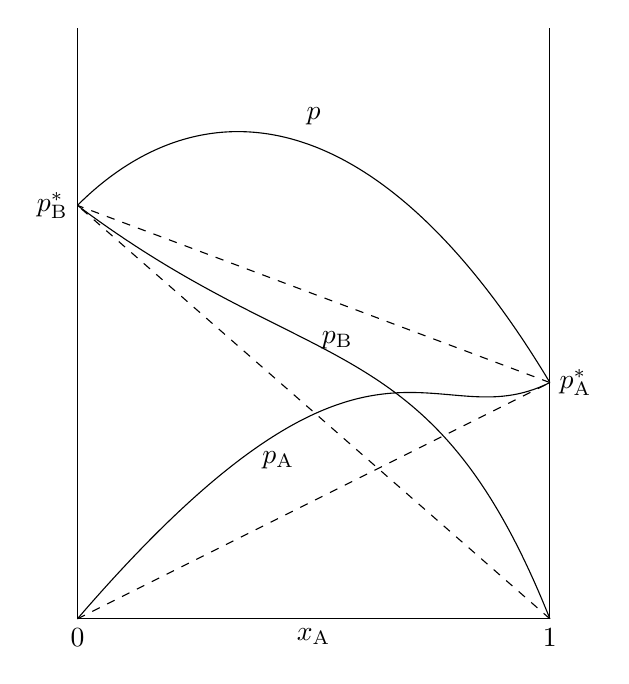
\begin{tikzpicture}[scale=1.5]
	\draw (-2.5,2) -- (-2.5,-3) node (v1) [below]{$0$} -- (1.5,-3) node (v2) [below]{$1$} -- (1.5,2);
	\draw[dashed](-2.5,-3) --  (1.5,-1) node [right] (v3) {$p^{*}_{\mathrm{A}}$};
	\draw[dashed](1.5,-3) --  (-2.5,0.5) node [left] (v4) {$p^{*}_{\mathrm{B}}$};
	\draw[dashed](1.5,-1) --  (-2.5,0.5);
	\node at (-0.5,-3) [below]{$x_{\mathrm{A}}$};
	\node at (1.5,-2) {};
	\draw (-2.5,-3);
	\draw (-2.5,-3) .. controls (0,-0.1) and (0.5,-1.5) .. (1.5,-1);
    \draw (-2.5,0.5) .. controls (-0.5,-1) and (0.5,-0.5) .. (1.5,-3);
    \draw (-2.5,0.5) .. controls (-1.5,1.5) and (0,1.5) .. (1.5,-1);
    \node at (-0.5,1.1)[above]{$p$};
    \node at (-0.8,-1.5)[below]{$p_{\mathrm{A}}$};
    \node at (-0.3,-0.8)[above]{$p_{\mathrm{B}}$};
   \end{tikzpicture}
   \end{center}
   
   The fact that a very dilute solute does not obey Raoult's law can be explained from a molecular point of view by the fact that in such dilute solution the solvent's molecules will be almost entirely surrounded by solvent molecules. Unless the solvent and the solute are very similar molecules (benzene-toluene), the properties of the solute will be strongly affected by the presence of the solvent.
   \subsection*{Phase diagrams}
   We have just seen that for a solution that obeys Raoul't law, an ideal solution, the total vapour pressure of the solution varies linearly with composition and the straight line that joins $p^{*}_{\mathrm{A}}$ and $p^{*}_{\mathrm{B}}$ is called the \textit{bubble line}. However this does not give us any information on the composition of the vapour phase. It is reasonable to expect that this will be richer in the more volatile of the 2 components, but can we calculate its composition? From Raoult's law we know the partial pressures of the 2 components of the solution and from \textit{Dalton's law} we know that the molar fraction of each component in the vapour phase is proportional to its partial pressure. For the 2 components A and B Dalton's law can be written as $y_{\mathrm{A}}=p_{\mathrm{A}}/{p}$ and $y_{\mathrm{B}}=p_{\mathrm{B}}/{p}$. With a few simple algebraic substitutions we obtain the value of $y_{\mathrm{A}}$ and $y_{\mathrm{B}}$:
   \begin{equation*}
   y_{\mathrm{A}}=\frac{x_{\mathrm{A}} p^{*}_{\mathrm{A}}}{p^{*}_{\mathrm{B}}+(p^{*}_{\mathrm{A}}-p^{*}_{\mathrm{B}})x_{\mathrm{A}}}
   \end{equation*}    
   and $y_{\mathrm{B}}= 1-y_{\mathrm{A}}$.
   
   We can plot the results and we obtain the \textit{dew line}, which is not linear. The combination of the bubble line and the dew line is a pressure-composition phase diagram. Above the bubble line we have the liquid phase. Below the dew line we have the vapour phase. Between the 2 lines we have coexistence of liquid and vapour.
   \begin{center}
    \begin{tikzpicture}[scale=2]
	\draw (-2.5,2)node [left]{$p$} -- (-2.5,-3) node (v1) [below]{$0$} -- (1.5,-3) node (v2) [below]{$1$} -- 		(1.5,2);
	\node at (1.5,-1)  [right] {$p^{*}_{\mathrm{A}}$};
	\node at (-2.5,1) [left] {$p^{*}_{\mathrm{B}}$};
	\draw[-] (-2.5,1)to node[sloped,midway,above] {bubble line} (1.5,-1);
	\node at (-0.5,-3) [below]{$x_{\mathrm{A}},y_{\mathrm{A}}$};
	\node at (1.5,-2) {};
	\draw (-2.5,1) ..  controls (-1.5,-0.5) and (0,-1) .. (1.5,-1) node[sloped,midway,below]{dew line};
    \node at (-0.5,1) {L};
    \node at (-0.5,-2) {V};
    \node at (-0.6,-0.3) {L+V};
    \end{tikzpicture}
   \end{center}
   By using a pressure-composition or $p-x$ diagram, we can easily calculate the composition of both phases for any isothermal change of pressure. If we started with a liquid solution represented by point 1 on the diagram and we reduced the pressure keeping the temperature constant until we reached point 2 on the bubble line, we could calculate the composition of the corresponding vapour phase. This can be achieved by simply moving to the dew line at the same pressure (point 2').
   \begin{center}
    \begin{tikzpicture}[scale=2]
	\draw (-2.5,2)node [left]{$p$} -- (-2.5,-3) node (v1) [below]{$0$} -- (1.5,-3) node (v2) [below]{$1$} -- 		(1.5,2);
	\node at (1.5,-1)  [right] {$p^{*}_{\mathrm{A}}$};
	\node at (-2.5,1) [left] {$p^{*}_{\mathrm{B}}$};
	\draw[-] (-2.5,1)to (1.5,-1);
	\node at (-0.5,-3) [below]{$x_{\mathrm{A}},y_{\mathrm{A}}$};
	\node at (1.5,-2) {};
	\draw (-2.5,1) ..  controls (-1.5,-0.5) and (0,-1) .. (1.5,-1);
	\draw[fill] (0.5,0.2) circle [radius=0.025];
	\draw[fill] (0.5,-0.5) circle [radius=0.025];
	\draw[fill] (-.82,-0.5) circle [radius=0.025];
    \draw[dashed] (0.5,0.2) node [left]{1} to (0.5,-0.5) node [right,yshift=0.15cm]{2};
    \draw[dashed] (0.5,-0.5) to (-.82,-0.5) node [above]{2'};
    \draw[dotted] (-.82,-0.5) to (-.82,-3) node [left,yshift=0.2cm]{$y_{\mathrm{A}}(2)$};
    \draw[dotted] (0.5,-0.5) to (0.5,-3) node [right,yshift=0.2cm]{$x_{\mathrm{A}}(2)$};
    \end{tikzpicture}
   \end{center}
   
   Often in chemical processes it's easier to achieve phase changes by changing the temperature keeping the pressure constant, rather than the other way around. In this case it is useful to represent phase equilibrium and the composition of the 2 phases at different temperatures. An example of these temperature-composition (or $T-x$) diagrams is shown in the following figure. 
   \begin{center}
    \begin{tikzpicture}[scale=2]
	\draw (-2.5,2)node [left]{$T$} -- (-2.5,-3) node (v1) [below]{$0$} -- (1.5,-3) node (v2) [below]{$1$} -- 		(1.5,2);

	\node at (-0.5,-3) [below]{$x_{\mathrm{A}},y_{\mathrm{A}}$};

	\draw (-2.5,-1) node [left]{$T^{*}_{\mathrm{B}}$} ..  controls (-1.5,-0.8) and (0,-1) .. (1.5,1) node[sloped,midway,below]{bubble line};
    \draw (-2.5,-1) ..  controls (-1.5,0.5) and (0,0.8) .. (1.5,1) node[sloped,midway,above]{dew line};
    \node at (-0.5,1) {V};
    \node at (-0.5,-1.5) {L};
    \node at (-0.6,-0.1) {L+V};
    \node at (1.5,1) [right]{$T^{*}_{\mathrm{A}}$};
    \end{tikzpicture}
   \end{center}
   
   In this case both lines are not linear. The bottom line is the bubble line and below it we have the liquid phase. The top line is the dew line and above it we have the vapour phase.
   \subsection*{Distillation}
   From phase diagrams it is easy to visualise that at the equilibrium between a solution and its vapour, the vapour will be richer in the more volatile of the 2 components. But if we could re-condensate this vapour, the resulting liquid phase  would also be richer in the more volatile of the 2 components. By repeating this cycle of evaporation and condensation several times it is possible to completely separate the 2 components of the initial solution. This is the working principle behind the distillation process.
   \begin{figure}[H]
   \begin{center}
    \begin{tikzpicture}[scale=1.3]
	\draw (-2.5,2)node [left]{$T$} -- (-2.5,-3) node (v1) [below]{$0$} -- (1.5,-3) node (v2) [below]{$1$} -- 		(1.5,2);

	\node at (-0.5,-3) [below]{$x_{\mathrm{A}},y_{\mathrm{A}}$};

	\draw (-2.5,-1) node [left]{$T^{*}_{\mathrm{B}}$} ..  controls (-1.5,-0.8) and (0,-1) .. (1.5,1)node [right]{$T^{*}_{\mathrm{A}}$} ;
    \draw (-2.5,-1) ..  controls (-1.5,0.5) and (0,0.8) .. (1.5,1);
    
    \draw[fill] (1.04,0.47) node (v3) {} circle [radius=0.025];
    \draw[fill] (-0.73,0.47) node (v4) {} circle [radius=0.025];
	\draw[fill] (-0.73,-0.68) node (v5) {} circle [radius=0.025];
	\draw[fill] (-2.27,-0.68) node (v6) {} circle [radius=0.025];

    \draw[dashed]  (v3)node [right]{1} -- (v4)node [left,yshift=0.1cm]{1'};
    \draw [dashed] (v5) -- (v4);
    \draw [dashed] (v5) node [right,yshift=-0.15cm]{2}  -- (v6)node [left]{2'};
    \end{tikzpicture}
   \includegraphics[scale=0.35]{Images/Lect2_distillation_column.pdf} 
   \end{center}
   \end{figure}
   \subsection*{Azeotropes}
   If the behaviour of a solution deviates strongly from that of an ideal solution its liquid-vapour phase diagram could look like the following figures.
   \begin{center}
    \begin{tikzpicture}[scale=1.5]
	\draw (-2.5,2)node [left]{$T$} -- (-2.5,-3) node (v1) [below]{$0$} -- (1.5,-3) node (v2) [below]{$1$} -- 		(1.5,2);

	\node at (-0.5,-3) [below]{$x_{\mathrm{A}},y_{\mathrm{A}}$};


    \draw (-2.5,-2) node (v3) {} ..  controls (-1.5,0.5) and (0,2.5) .. (1.5,1);
    \draw  plot[smooth, tension=.7] coordinates {(v3)};
    \node at (0.42,1.52) {};
    \draw (-2.49,-1.99)node[left]{$T^{*}_{\mathrm{B}}$} .. controls (-1.67,-2.12) and (-0.08,1.7) .. (0.42,1.51);
    \draw (0.43,1.51) .. controls (0.81,1.5) and (1.13,0.9) .. (1.48,1) node[right]{$T^{*}_{\mathrm{A}}$};
    \end{tikzpicture}
    \begin{tikzpicture}[scale=1.5]
	\draw (-2.5,2)node [left]{$T$} -- (-2.5,-3) node (v1) [below]{$0$} -- (1.5,-3) node (v2) [below]{$1$} -- 		(1.5,2);

	\node at (-0.5,-3) [below]{$x_{\mathrm{A}},y_{\mathrm{A}}$};
    \draw (-2.5,-2) .. controls (-1.,-3.) and (1,-3.33) .. (1.49,0.99);
    \node at (-0.69,-2.62) {};
    \draw (-2.49,-1.99) node[left]{$T^{*}_{\mathrm{B}}$} .. controls (-1.97,-1.88) and (-1.08,-2.71) .. (-0.69,-2.62);
    \draw (-0.69,-2.62) .. controls (0.42,-2.68) and (1.19,1.16) .. (1.49,0.98)node[right]{$T^{*}_{\mathrm{A}}$} ;
    \end{tikzpicture}
   \end{center}
   
   In this case it is not possible to separate the mixture into its components by distillation. The solution forms an \textbf{azeotrope}: the liquid and the vapour phase have the same composition and the distillation is not able to proceed any further.
   \subsection*{Chemical potential}
   How can we fit ideal and real solutions in the picture of thermodynamics that we have drawn so far? We have initially defined the internal energy of a system $U$ and subsequently we have introduced the work of expansion and contraction and the state function enthalpy $H$. Then we discussed entropy $S$ and finally we combined all these different thermodynamical drivers into the definition of Gibbs free energy $G$. What's missing in order to complete the picture is something dependent on the amount of substance\footnote{Actually the electrochemical potential is also missing, and it will be discussed in a different part of this module.}. We define the \textbf{chemical potential} of a pure substance as:
   \begin{equation*}
   \mu = \left(\frac{\partial G}{\partial n}\right)_{T,p}
   \end{equation*}
   which is the variation in Gibbs free energy caused by an infinitesimal change of amount of substance, when temperature and pressure remain constant. So, in the case of a pure substance, the chemical potential is the molar free energy.
   For a perfect gas:
   \begin{equation*}
   \mu =\mu^{\standardstate}+RT\ln\frac{p}{p^{\standardstate}} 
   \end{equation*}
   Similarly we can define the chemical potential for a multi-component system as:
   \begin{equation*}
   \mu_{i} = \left(\frac{\partial G}{\partial n_{i}}\right)_{T,p,n_{j\neq i}}
   \end{equation*}
   which is the variation in Gibbs free energy caused by an infinitesimal change of amount of substance $i$, when temperature, pressure and amount of all other substances remain constant. Alternatively we could say that the chemical potential, in a multi-component system, is the partial molar free energy.
   In an ideal solution: 
  \begin{equation*}
  \mu_{i,\mathrm{l}} =\mu^{*}_{i,\mathrm{l}}+RT\ln x_{i} 
  \end{equation*}
  where $\mu^{*}_{i,\mathrm{l}}$ is the chemical potential of pure component $i$.
  If a solution does not follow Raoult's law, the deviation from ideality can be expressed introducing the activity of species $i$, definded as $a_{i}=\gamma_{i} x_{i}$. The previous equation becomes:
  \begin{equation*}
  \mu_{i,\mathrm{l}} =\mu^{*}_{i,\mathrm{l}}+RT\ln a_{i} 
  \end{equation*}
  Why is chemical potential important in the study of thermodynamical equilibrium? Because it contains information about how changes of system composition affect the state of equilibrium. For a system to be in equilibrium the chemical potential $\mu_{i}$ of each species $i$ must be the same in each part of the system.
  \subsection*{Solubility}
  We can use the concept of chemical potential to calculate the solubility of a solid solute in a solvent. We consider the pure solid species A, the solute, in equilibrium with a solution containing the solute and a solvent. In such state of equilibrium the chemical potential of the solute in the 2 phases must be the same. We can express this as:
   \begin{equation*}
   \mu_{\mathrm{A,solution}}(T,p,x_{\mathrm{A}}) = \mu_{\mathrm{A,solid}}(T,p)
   \end{equation*} 
   which we can write as:
   \begin{equation*}
   \mu^{*}_{\mathrm{A}}(T,p)+RT\ln x_{\mathrm{A}} = \mu_{\mathrm{A,solid}}(T,p)
   \end{equation*} 
   where $\mu^{*}_{\mathrm{A}}(T,p)$ is the chemical potential of A as a pure liquid. We can rearrange this equation as:
   \begin{equation*}
   \ln x_{\mathrm{A}} = -\frac{\mu^{*}_{\mathrm{A}}(T,p)-\mu_{\mathrm{A,solid}}(T,p)}{RT}
   \end{equation*} 
   The term $\mu^{*}_{\mathrm{A}}(T,p)-\mu_{\mathrm{A,solid}}(T,p)$ is the Gibbs free energy of fusion of species A, so we can write this as:
   \begin{equation*}
   \ln x_{\mathrm{A}} = -\frac{\Delta G_{\mathrm{A,fus}}}{RT}
   \end{equation*} 
   We would like to calculate the value of $x_{\mathrm{A}}$ as a function of temperature. A full derivation of the following results would have to make use of the \textbf{Gibbs-Helmholtz equation}, which we will derive during one of the following lectures. Therefore, at this stage I will simply show you the resulting equation while the complete derivation will be shown at a later stage. The solubility at temperature $T$ is given by:
   \begin{equation*}
   \ln x_{\mathrm{A}} = -\frac{\Delta H_{\mathrm{A,fus}}}{R}(\frac{1}{T}-\frac{1}{T^{*}_{\mathrm{A}}})
   \end{equation*}
where $T^{*}_{\mathrm{A}}$ is the melting point of species A.
\end{document}